% You can choose whether you prefer a single or double column appendix.
% Whatever you choose, you will need to stick to it throughout the appendix.
% For double column style, comment the next line.
\onecolumn

\appendix
\begin{appendices}

\section{Acknowledgements}
\label{appendix:acknowledgements}

My sincere gratitude to all the participants who generously contributed to this study by dedicating their time to respond to the surveys and questionnaires voluntarily, as well as those who willingly tested and interacted with the prototype. Special appreciation goes to everyone who supported me in data analysis, provided hardware for the prototypes, and reviewed and tested the code for the hardware devices.

A thank you to supervisor, Dr. H. Seiied Alavi (University of Amsterdam), for his invaluable guidance, thought-provoking questions, and overall assistance throughout the project and Shruti Rao PhD Candidate (University of Amsterdam) for her constructive feedback and suggestions, which further expanded this research. Also, my sincere appreciation to all the reviewers of this research for their insightful comments and contributions.

\section{Ethical considerations}
\label{appendix:ethical}

Before user studies were conducted, an application to the Ethics Committee for Information Sciences (ECIS) \footnote{https://ivi.uva.nl/research/ethical-code/ethical-code.html} about the methodology of this research, how data is being gathered and stored was made. Advice from the committee is still pending.

All individuals participating in the survey and evaluation process were obliged to confirm their voluntary involvement by carefully reading and signing a letter of consent, with the assurance that they retained the right to withdraw from participation at any point without the need for explanation. Participants were informed about the goal of the study and the structure of the interviews. To uphold confidentiality and privacy, survey participation occurred anonymously, and all evaluation interview data underwent anonymization following the conclusion of the evaluation sessions.

Interacting with occupants within the building and interacting with participants of the usability tests of the prototype adhered to the the principles outlined in the UvA code of conduct \footnote{https://www.uva.nl/en/about-the-uva/policy-and-regulations/}.

\section{Domain Expert Validity}
\label{appendix:experts}

Prior to conducting the questionnaire survey and evaluation procedure, a domain expert from the Informatics Institute at the University of Amsterdam reviewed the methodologies involved. First versions were send out to staff for feedback internally. The surveys and interviews were tested internally as pilot tests and then distributed to participants and open for participation. 

\section{Data storage and archival}
\label{appendix:data}

Take some parts of the ethical application to describe data storage and archival of the devices etc.

\section{Source code}
\label{appendix:source}

In the spirit of open research, to support reproducibility and replication, to mitigate a lack of transparency, and to enable future work in this research field the datasets, notebooks, and prototypes in this work are publicly available on a GitHub organization with the working title 'viszlab' \footnote{https://github.com/viszlab} using the MIT License. Several code repositories for different parts of the research can be accessed. The readme of the repository described the contents and how to perform the technical set-up:

\begin{enumerate}
  \item \textbf{Prototype}. Code and models for the physical prototype.\\
  \underline{https://github.com/viszlab/prototype}
  \item \textbf{Datasets}. Code and models for the physical prototype.\\
  \underline{https://github.com/viszlab/prototype}
\end{enumerate}

A one-page website was created for shareability of this research. It's an online website which gives an overview of the research, allows for viewing the source coded of the prototype and allows for downloading of this paper. A live version is deployed on:

\begin{enumerate}
  \item \textbf{One-pager}. Code and models for the physical prototype.\\
  \underline{https://viszlab.github.io/}
\end{enumerate}

\pagebreak

\section{Floorplan and lab set-up}
\label{appendix:floorplan}

A diagram indicating where the sensors where installed. This shows the lab set-up in the two meeting rooms.

\begin{figure}[H]
    \centering
    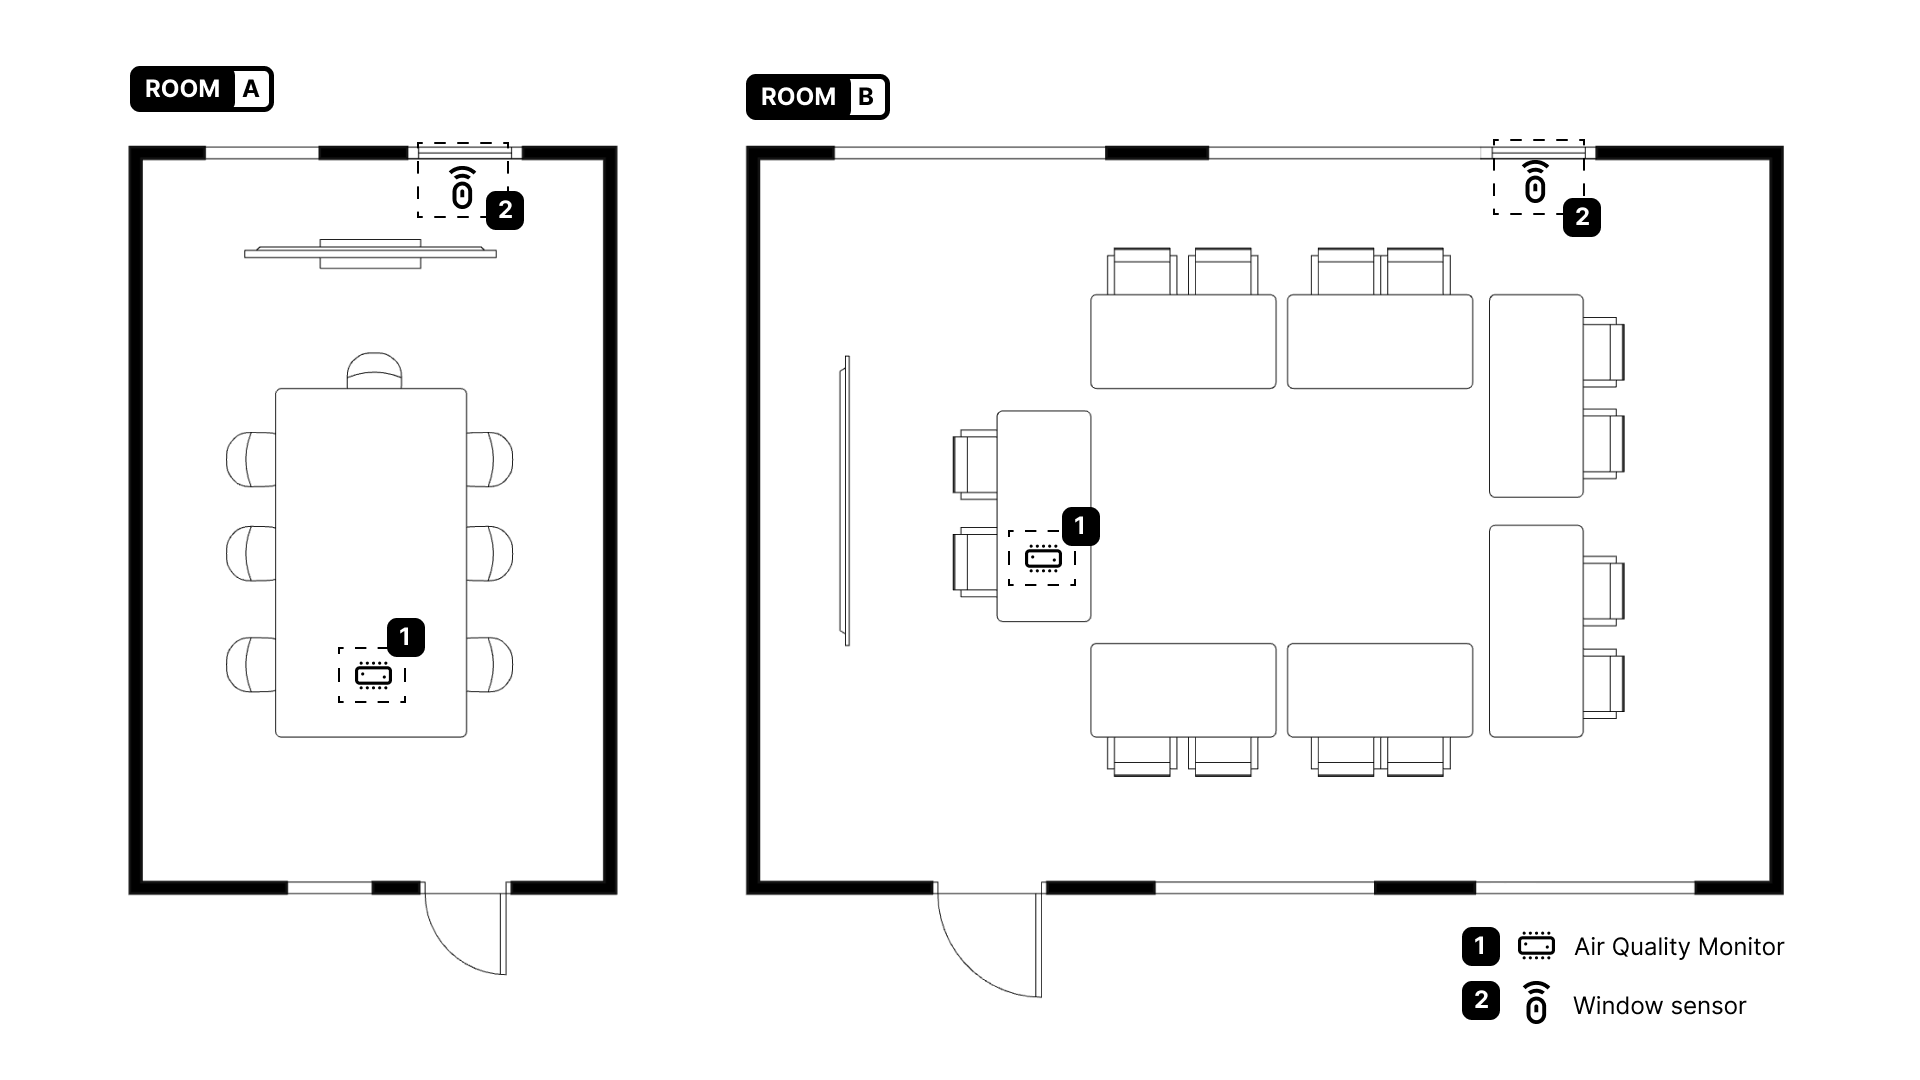
\includegraphics[width=0.6\paperwidth]{floorplan.png}
    \caption{Diagram of the floorplan with sensors installed}
    \label{fig:timeline}
\end{figure}

\section{IoT architecture of the prototype}
\label{appendix:architecture}

System diagram which shows the IoT architecture of the prototype.

\begin{figure}[H]
    \centering
    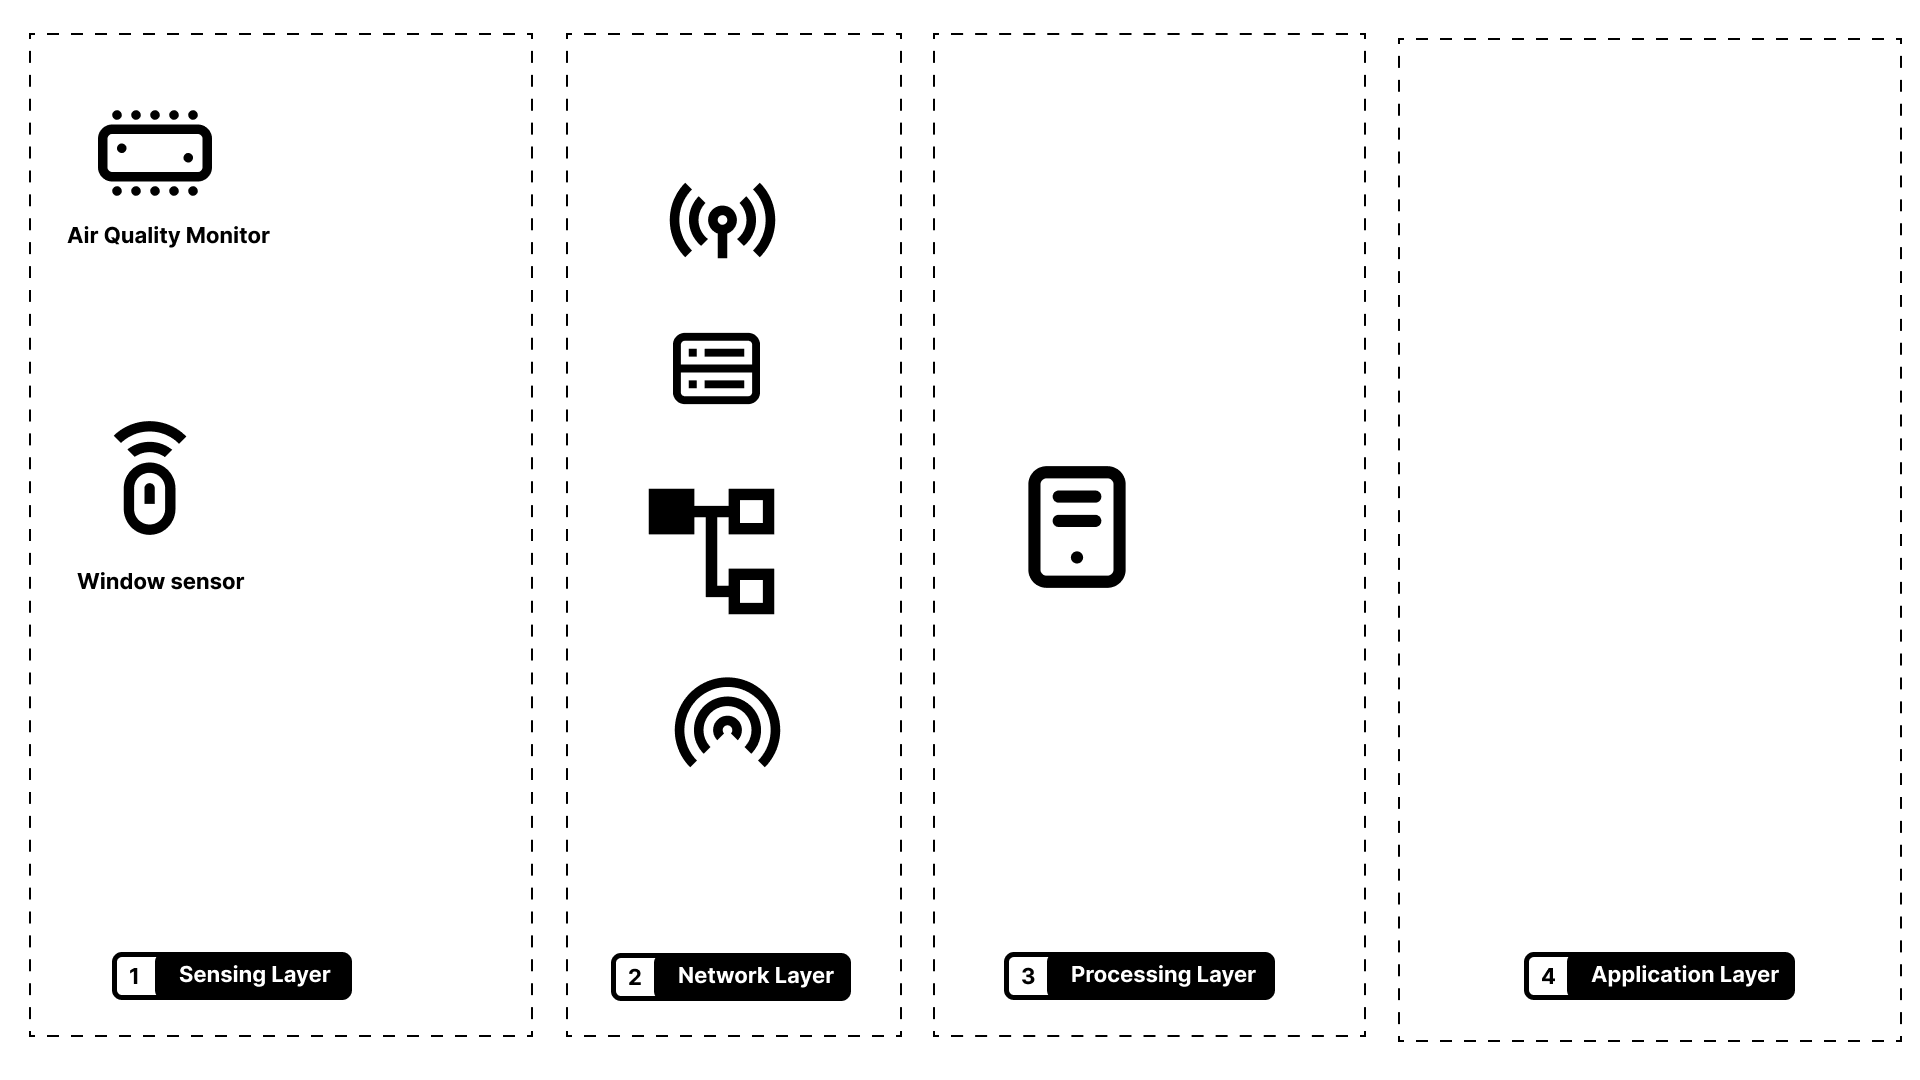
\includegraphics[width=0.7\paperwidth]{system.png}
    \caption{System diagram that shows the technical set-up of the prototype}
    \label{fig:timeline}
\end{figure}

\pagebreak

\section{Meeting room impressions}
\label{appendix:meetings}

\begin{figure}[H]
\begin{minipage}{.5\textwidth}
    \centering
    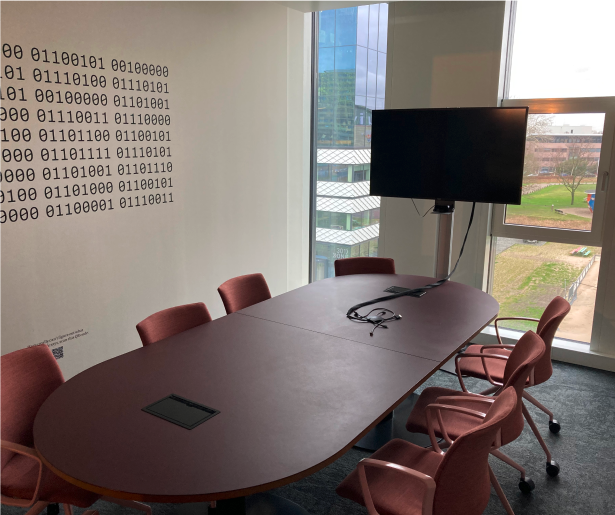
\includegraphics[width=80mm,height=80mm]{building.png}
    \caption{System diagram that shows the }
    \label{fig:timeline}
\end{minipage}%
\begin{minipage}{.5\textwidth}
    \centering
    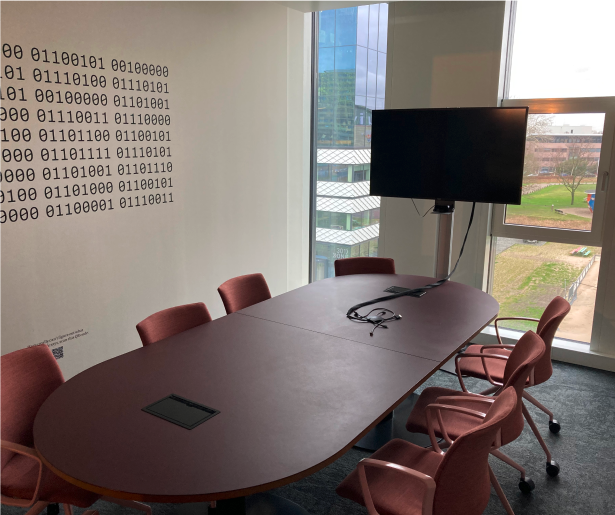
\includegraphics[width=80mm,height=80mm]{building.png}
    \caption{System diagram that shows the }
    \label{fig:timeline}
\end{minipage}%
\end{figure}

\section{Building impressions}
\label{appendix:building}

\begin{figure}[H]
\begin{minipage}{.5\textwidth}
\begin{tabular}{cc}
  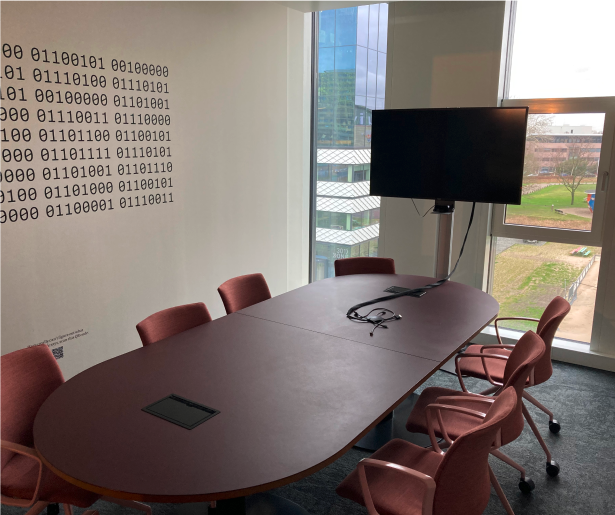
\includegraphics[width=45mm]{building.png} &   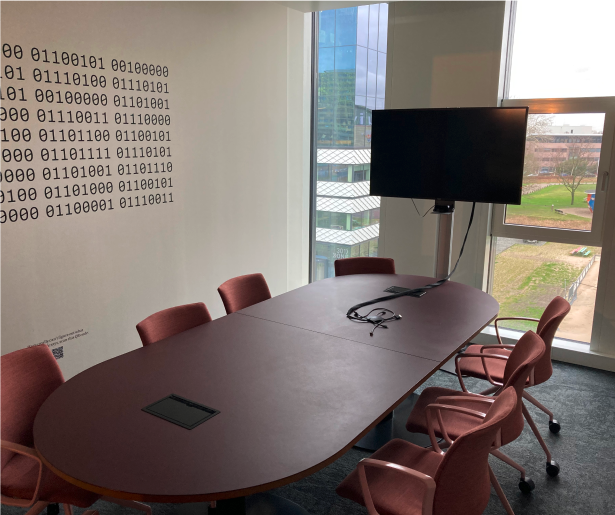
\includegraphics[width=45mm]{building.png} \\
(a) first & (b) second \\[6pt]
 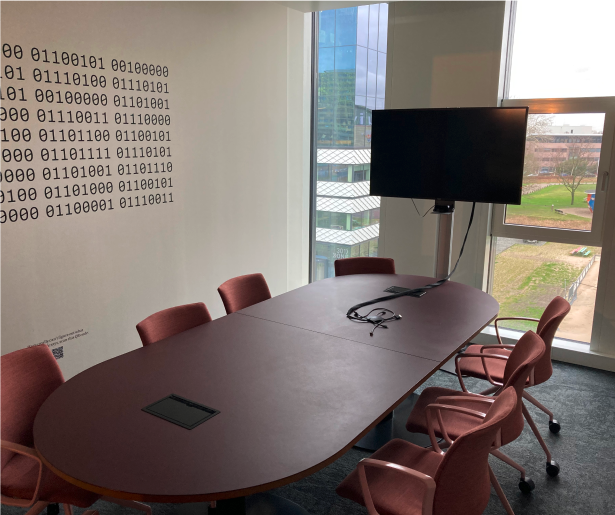
\includegraphics[width=45mm]{building.png} &   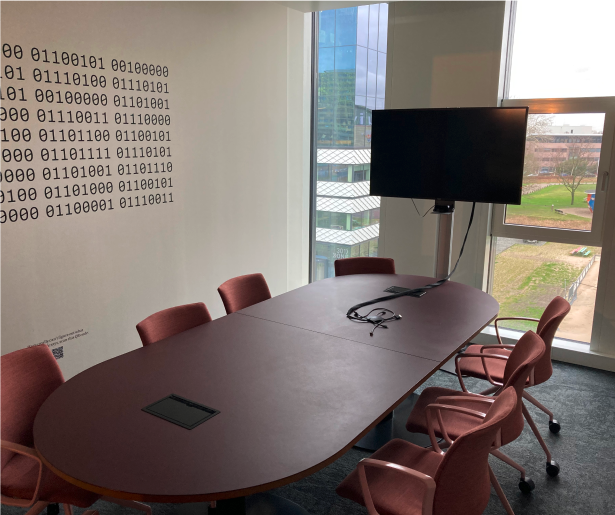
\includegraphics[width=45mm]{building.png} \\
(c) third & (d) fourth \\[6pt]
\end{tabular}
\caption{caption}
\end{minipage}%
\begin{minipage}{.5\textwidth}
    \centering
    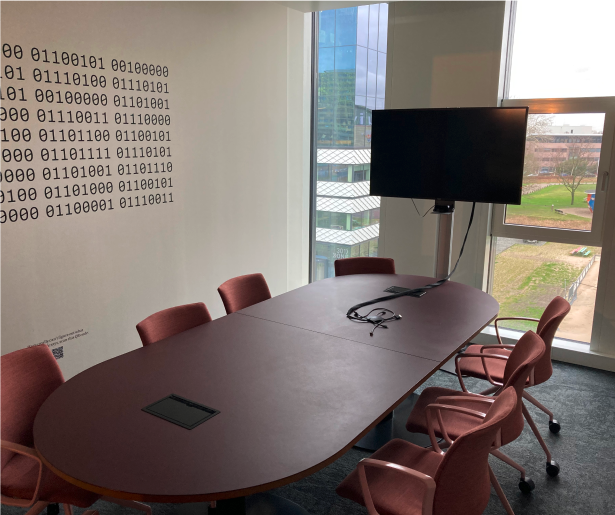
\includegraphics[width=70mm,height=80mm]{building.png}
    \caption{System diagram that shows the }
    \label{fig:timeline}
\end{minipage}%
\end{figure}

\section{Prototype impressions}
\label{appendix:prototype}

\begin{figure}[H]
\begin{minipage}{.5\textwidth}
    \centering
    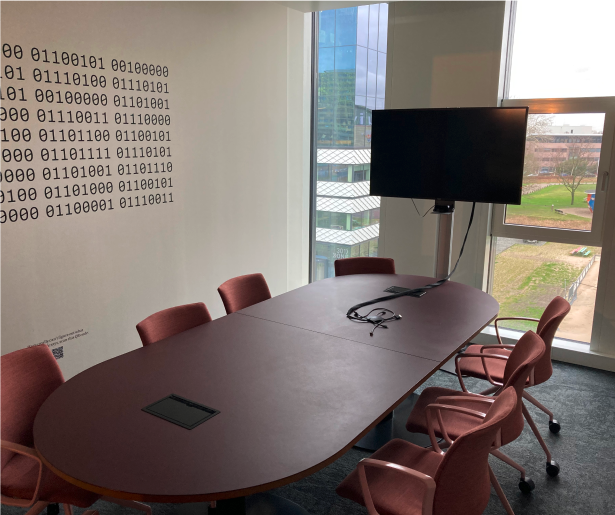
\includegraphics[width=70mm,height=80mm]{building.png}
    \caption{System diagram that shows the }
    \label{fig:timeline}
\end{minipage}%
\begin{minipage}{.5\textwidth}
\begin{tabular}{cc}
  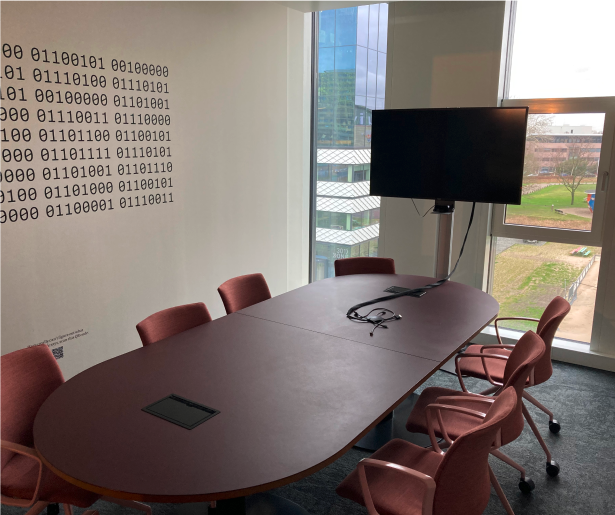
\includegraphics[width=45mm]{building.png} &   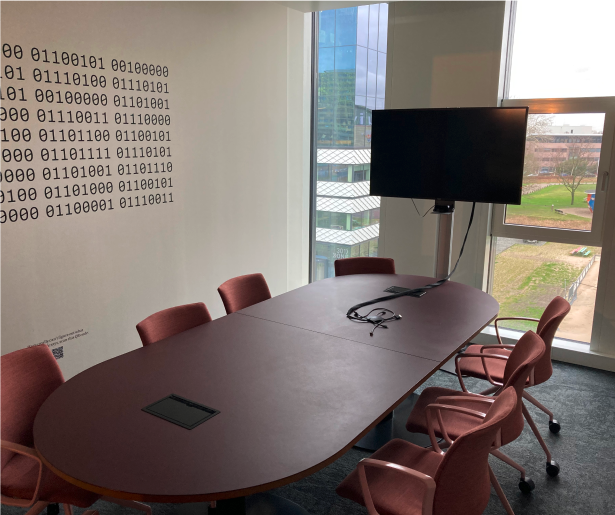
\includegraphics[width=45mm]{building.png} \\
(a) first & (b) second \\[6pt]
 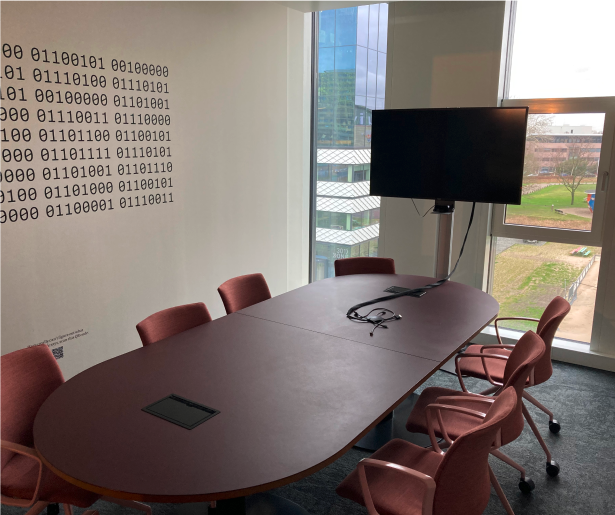
\includegraphics[width=45mm]{building.png} &   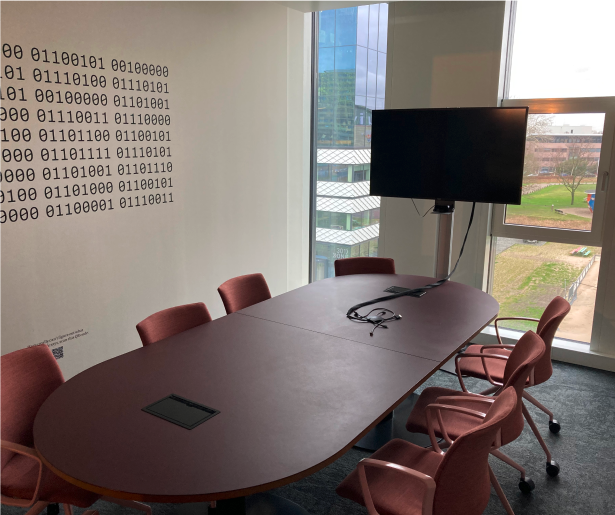
\includegraphics[width=45mm]{building.png} \\
(c) third & (d) fourth \\[6pt]
\end{tabular}
\caption{caption}
\end{minipage}%
\end{figure}

\section{Weekly schedule}
\label{appendix:schedule}

Horizontal boxplot that indicates an average week of booking in the meeting rooms scheduled.

\begin{figure}[H]
    \centering
    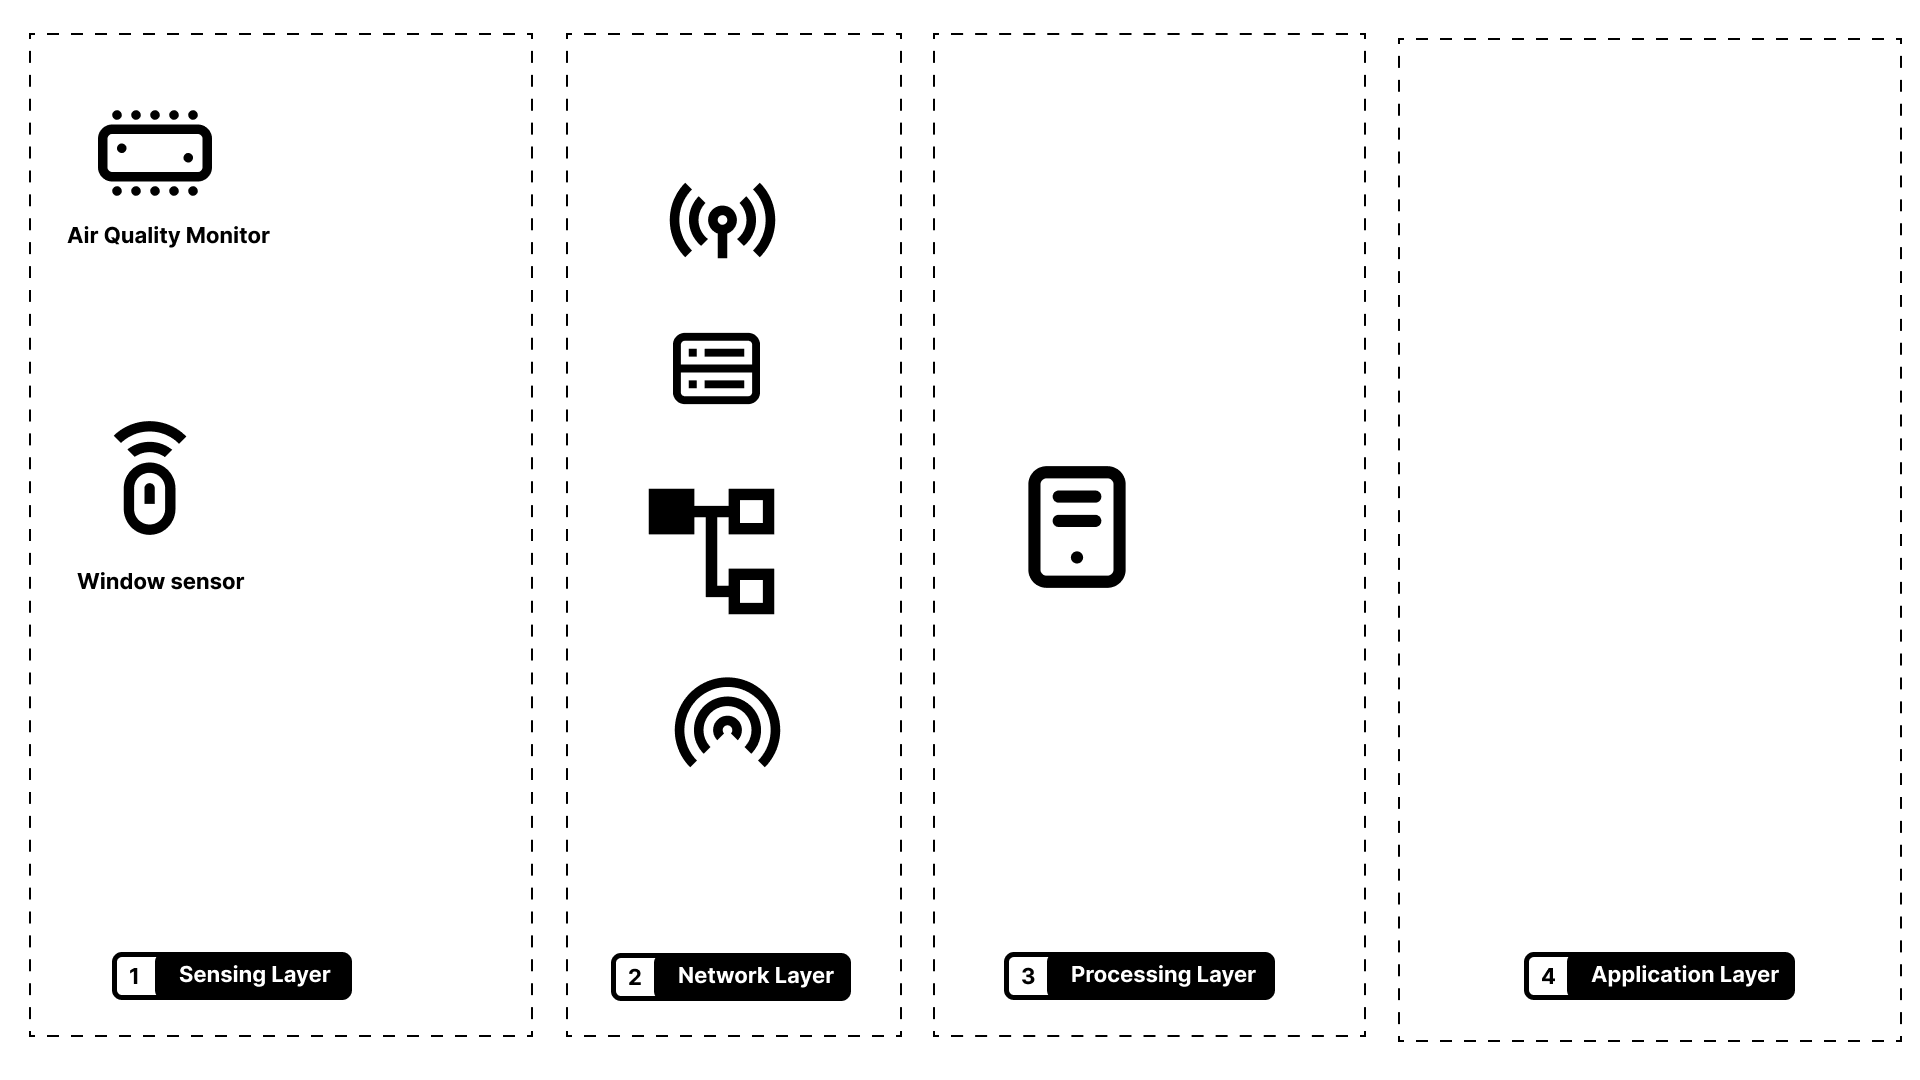
\includegraphics[width=0.7\paperwidth]{system.png}
    \caption{System diagram that shows the technical set-up of the prototype}
    \label{fig:timeline}
\end{figure}

\pagebreak

\section{Air Quality Monitors sample data}
\label{appendix:monitors}

\section{Questionnaire survey (POE)}
\label{appendix:survey}

\textbf{Introduction:}\\

Hi! We at the Digital Interactions Lab (DIL) are researching indoor environments, focusing on Indoor Air Quality (IAQ) within smart buildings like Lab42, for a Master Thesis. This survey takes an average of $\sim$3 minutes to complete and comprises questions about your overall comfort and awareness of Indoor Air Quality (IAQ).

The survey is anonymous and collects data on environmental experiences and approximate building location for future research and publication.

\textbf{Informed constent:}\\
Participation is voluntary, and if you decide that you do not want to participate after you have completed it, please contact us.

\textbf{Contact details:}\\
Principal researcher: BSc D. de Vries - \href{mailto:danny.de.vries@student.uva.nl}{danny.de.vries@student.uva.nl}

Supervisor(s): Shruti Rao PhD Candidate - \href{mailto:s.rao@uva.nl}{s.rao@uva.nl}

Supervisor(s): Dr. H. Seiied Alavi PhD - \href{mailto:ha.alavi@uva.nl}{ha.alavi@uva.nl}

Thank you for your valuable time and for participating in our survey!\\\\

\textbf{Q1: Location}- Where are you currently located within the Lab42 building?

\begin{itemize}
    \item On the ground floor (the atrium)
    \item On the first floor (1st floor - in a working space)
    \item On the second floor (2nd floor - in a working space)
\end{itemize}

\textbf{Q2: Activity} - On average, how often do you use Lab42 per week for various activities?

\begin{itemize}
    \item 1 day a week
    \item 2 days a week
    \item 3 days a week
    \item 4 days a week
    \item 5 days a week
\end{itemize}

\textbf{Q3: Occupancy} - How would you describe the occupancy in your current space?

\begin{itemize}
    \item Not crowded
    \item Not too crowded
    \item Crowded
    \item Very crowded
    \item At capacity
\end{itemize}

\textbf{Q4: Awareness Air Quality} - Did you know that poor air quality has been identified to pose health risks and affect cognitive performance? How aware are you of the current air quality in this space?

\textbf{Q6: Perceived Air Quality} - How do you perceive the air quality in the current space?

\textbf{Q7: Satisfaction Air Quality} - How satisfied are you with the air quality in the current space?

\textbf{Q8: Not mandatory} - Would you like to describe in more detail in your own words how you currently feel about the Indoor Air Quality?

\textbf{Q9: Health symptoms} - Do you experience any health-related symptoms based on the air quality in this space?

\begin{itemize}
    \item None
    \item Headaches
    \item Trouble breathing
    \item Feeling nauseating
    \item Other
\end{itemize}

\textbf{Q10: Cognitive symptoms} - Do you experience any cognitive-based symptoms on the air quality in this space?

\begin{itemize}
    \item None
    \item Trouble with focus
    \item Decreased productivity
    \item Tiredness
    \item Other
\end{itemize}


\section{Harris profile}
\label{appendix:profile}


\begin{table}[h]
    \centering
    \begin{tabularx}{\textwidth}{|c|*{12}{X|}}
        \hline
        & \multicolumn{4}{c|}{Concept 1} & \multicolumn{4}{c|}{Concept 2} & \multicolumn{4}{c|}{Concept 3} \\
        \cline{2-13}
        Requirements & -2 & -1 & +1 & +2 & -2 & -1 & +1 & +2 & -2 & -1 & +1 & +2 \\
        \hline
        Row 1 & & & & & & & & & & & & \\
        \hline
        Row 2 & & & & & & & & & & & & \\
        \hline
        Row 3 & & & & & & & & & & & & \\
        \hline
        Row 4 & & & & & & & & & & & & \\
        \hline
        Row 5 & & & & & & & & & & & & \\
        \hline
        Row 6 & & & & & & & & & & & & \\
        \hline
        Row 7 & & & & & & & & & & & & \\
        \hline
        Total Score & \multicolumn{4}{c|}{Total} & \multicolumn{4}{c|}{Total} & \multicolumn{4}{c|}{Total} \\
        \hline
    \end{tabularx}
    \caption{Harris profile for the three concepts models to visualize the strengths and weaknesses of the design concepts.}
    \label{tab:requirements_table}
\end{table}

\section{Expert reviews}
\label{appendix:expert}

\section{Evaluation Interviews}
\label{appendix:evaluation}

\section{Usability tests}
\label{appendix:usability}

\section{Effectiveness scores}
\label{appendix:effectiveness}

\section{Academic sample case studies}
\label{appendix:academic}

In the ideation phase and development of concept models, seven academic publications were instrumental in informing and inspiring the design process. Table 1 provides an overview of these publications, presenting details such as the title, authors, publication year, and relevant venue.

\begin{table}[htbp]
\centering
\caption{Overview of the 7 academic case studies used for the ideation phase and concept models.}
\label{tab:my-table}
\begin{tabularx}{\textwidth}{|>{\raggedright\arraybackslash}m{1cm}|X|X|>{\raggedright\arraybackslash}m{1cm}|X|X|}
\hline
\textbf{Nr.} & \textbf{Sample} & \textbf{Author(s)} & \textbf{Year} & \textbf{Venue} & \textbf{Reference} \\ \hline
1 & Econundrum & Unknown & Unknown & non-academic & \href{https://dl.acm.org/doi/10.1145/3357236.3395509}{Econundrum} \\ \hline
2 & Caimform & Unknown & Unknown & non-academic & \href{http://dataphys.org/list/cairnform-a-physical-ring-chart-showing-renewable-energy-data/}{Caimform} \\ \hline
3 & Dataponics & Unknown & Unknown & non-academic & \href{http://dataphys.org/list/dataponics-human-vegetal-play/}{Dataponics} \\ \hline
4 & Garden of Eden & Unknown & Unknown & non-academic & \href{http://dataphys.org/list/garden-of-eden/}{Garden of Eden} \\ \hline
5 & Pudica & Unknown & Unknown & non-academic & \href{https://trackr-media.tangiblemedia.org/publishedmedia/Papers/715-MTA0N/Published/PDF}{Pudica} \\ \hline
6 & ComfortBox & Hamed S. Alavi et al. & 2017 & IFIP & \href{https://doi.org/10.1007/978-3-319-67687-6_16}{ComfortBox} 
\\ \hline
7 & ComFeel & Ugo Sassi et al. & 2020 & ACM & \href{https://dl.acm.org/doi/10.1145/3432234}{ComFeel} 
\\ \hline
8 & WindowWall & Patrick Bader et al. & 2020 & ACM & \href{https://doi.org/10.1145/3310275}{WindowWall} \\ \hline
9 & Ambient Influence & Yvonne Rogers et al. & 2010 & ACM & \href{https://dl.acm.org/doi/10.1145/1864349.1864372}{Ambient Influence} 
\\ \hline
\end{tabularx}
\end{table}

\section{Non-academic sample case studies}
\label{appendix:nonacademic}

In the ideation phase and development of concept models, an exploration of non-academic case studies were instrumental in informing and inspiring the design process. Table 2 presents an overview of the 15 non-academic case studies. Each entry in the table includes essential details such as the title, creator, publication year, and a brief description of the case study's venue.

\begin{table}[htbp]
\centering
\caption{Overview of the 28 non-academic case studies used for the ideation phase and concept models.}
\label{tab:my-table}
\begin{tabularx}{\textwidth}{|>{\raggedright\arraybackslash}m{1cm}|X|X|>{\raggedright\arraybackslash}m{1cm}|X|X|}
\hline
\textbf{Nr.} & \textbf{Sample} & \textbf{Creator} & \textbf{Year} & \textbf{Venue} & \textbf{Reference} \\ \hline
1 & Birdie Design & Birdie Design & 2024 & non-academic & \href{https://www.bir.die/}{www.bir.die} \\ \hline
2 & Fields of Informality & Zhestkov & 2024 & non-academic & \href{https://www.artco.m.com/}{www.artco.m} \\ \hline
3 & Tree of Ténéré & Studio Drift & 2024 & non-academic & \href{https://studiodr.ift.com/}{www.studiodr} \\ \hline
4 & Kinetic Sculpture & ART+COM & 2024 & non-academic & \href{https://artco.m.com/}{www.artco.m} \\ \hline
5 & Electro Magnetic Field & Unknown & 2024 & non-academic & - \\ \hline
6 & Microsurgical Robot & Unknown & 2024 & non-academic & - \\ \hline
7 & Wind 3.0 & Studio Roosegaarde & 2024 & non-academic & \href{https://www.studior.oo/}{www.studior} \\ \hline
8 & Floralis Generica & Eduardo Catalano & 2024 & non-academic & - \\ \hline
9 & Lucid Stead & Phillip K. Smith III & 2024 & non-academic & - \\ \hline
10 & Flylight & Studio Drift & 2024 & non-academic & - \\ \hline
11 & Spectra 2 & FIELD & 2024 & non-academic & - \\ \hline
12 & Meadow & Studio Drift & 2024 & non-academic & - \\ \hline
13 & Wind Pavilion & Studio Roosegaarde & 2024 & non-academic & - \\ \hline
14 & Pet Lamp & Álvaro Catalán & 2024 & non-academic & - \\ \hline
15 & Living map & Unknown & Unknown & non-academic & \href{https://www.behance.net/gallery/68572509/LIVING-MAP}{Living map} \\ \hline
16 & Harassment plants & Unknown & Unknown & non-academic & \href{https://luizaugustomm.github.io/pages/harassment-plants.html}{Harassment plants} \\ \hline
17 & Popsicles of Pollution & Unknown & Unknown & non-academic & \href{https://www.theguardian.com/cities/gallery/2017/sep/01/popsicles-pollution-ice-lollies-taiwan-taipei-contaminated-waterways}{Popsicles of Pollution} \\ \hline
18 & Yellow Dust & Unknown & Unknown & non-academic & \href{http://yellowdust.intheair.es/}{Yellow Dust} \\ \hline
19 & Touching air & Unknown & Unknown & non-academic & \href{https://www.stefanieposavec.com/airtransformed}{Touching air} \\ \hline
20 & Physical Weather Display & Unknown & Unknown & non-academic & \href{https://www.boredpanda.com/weather-forecast-box-tempescope-ken-kawamoto/}{Physical Weather Display} \\ \hline
21 & Inequalities Quipu & Unknown & Unknown & non-academic & \href{https://tuteja.info/inequalities-quipu/}{Inequalities Quipu} \\ \hline
22 & Summer in the city & Unknown & Unknown & non-academic & \href{https://www.carolabartsch.ch/en/projects/dataviz}{Summer in the city} \\ \hline
23 & WeatherWindow & Unknown & Unknown & non-academic & \href{http://dataphys.org/list/weatherwindow/}{WeatherWindow} \\ \hline
24 & Point cloud & Unknown & Unknown & non-academic & \href{https://www.jamesleng.net/pointcloud/}{Point cloud} \\ \hline
25 & Tele-present water & Unknown & Unknown & non-academic & \href{https://www.dwbowen.com/telepresentwater/}{Tele-present water} \\ \hline
26 & Real-time Warning & Unknown & Unknown & non-academic & \href{https://vimeo.com/35520114}{Real-time Warning} \\ \hline
27 & airFIELD & Unknown & Unknown & non-academic & \href{http://dataphys.org/list/ecloud-airfield-ambient-airport-visualizations/}{airFIELD} \\ \hline
28 & Shanghai Spheres & Unknown & Unknown & non-academic & \href{https://www.taittowers.com/work?sort=newest}{Shanghai Spheres} \\ \hline
\end{tabularx}
\end{table}

\section{fabrication Techniques}
\label{appendix:fabrication}

\begin{table}[!htbp]
\centering
\caption{Overview of the 4 academic and 6 non-academic sample case studies used as inspiration for fabrication of the prototype.}
\label{tab:my-table}
\begin{tabularx}{\textwidth}{|>{\raggedright\arraybackslash}m{1cm}|X|X|>{\raggedright\arraybackslash}m{1cm}|X|X|}
\hline
\textbf{Nr.} & \textbf{Sample} & \textbf{Author(s)} & \textbf{Year} & \textbf{Venue} & \textbf{Reference} \\ \hline
1 & FibeRobo & Jack Forman et al. & 2023 & MIT Media Lab (TGM) & \href{https://trackr-media.tangiblemedia.org/publishedmedia/Papers/728-MTA2O/Published/PDF}{TGM} \\ \hline
2 & DefeXtiles & Jack Forman et al. & 2020 & MIT Media Lab (TGM) & \href{https://trackr-media.tangiblemedia.org/publishedmedia/Papers/703-MTAyN/Published/PDF}{TGM} \\ \hline
3 & Cilllia & Jifei Ou et al. & 2016 & MIT Media Lab (TGM) & \href{https://trackr-media.tangiblemedia.org/publishedmedia/Papers/703-MTAyN/Published/PDF}{TGM} \\ \hline
4 & UniMorph & Felix Heiberg et al. & 2015 & MIT Media Lab (TGM) & \href{https://trackr-media.tangiblemedia.org/publishedmedia/Papers/703-MTAyN/Published/PDF}{TGM} \\ \hline
5 & Geometric Floating Fabric & Billie Ruben & 2020 & non-academic & \href{https://www.printables.com/en/model/42342-geometric-floating-fabric-printed-necklace-by-bill}{Printables} \\ \hline
6 & Print On Fabric & Damien Jorrand & 2021 & non-academic & \href{https://than.gs/m/14347}{Thangs} \\ \hline
7 & Nasa Fabric Mk3 & John Bowler & 2018 & non-academic & \href{https://www.thingiverse.com/thing:3095799}{Thingiverse} \\ \hline  
8 & Servo Flower & Job Smolders & 2018 & non-academic & \href{https://pinshape.com/items/41182-3d-printed-servo-flower}{Pinshape} \\ \hline
9 & Multiuse Flexible Fabric & Posix & 2024 & non-academic & \href{https://www.printables.com/model/88579-multiuse-flexible-fabric}{Printables} \\ \hline
10 & Leaf Decorative Holder & Trilobyte3D & 2022 & non-academic & \href{https://www.printables.com/model/230363-leaf-drink-coasters-with-decorative-plant-holder}{Printables} \\ \hline
\end{tabularx}
\end{table}

\end{appendices}
